\documentclass[a4paper]{article}

\setlength{\oddsidemargin}{-1in}
\addtolength{\oddsidemargin}{0.05 \paperwidth}
\setlength{\evensidemargin}{-1in}
\addtolength{\evensidemargin}{0.05 \paperwidth}
\setlength{\textwidth}{0.9 \paperwidth}

\setlength{\topmargin}{-0.75in}
\addtolength{\topmargin}{0.05 \paperheight}
\setlength{\textheight}{\paperheight}
\setlength{\headheight}{0in}
\setlength{\headsep}{0in}
\setlength{\footskip}{0in}

\usepackage[T1]{fontenc}
\usepackage[utf8]{inputenc}
\usepackage[german]{babel}

\usepackage[default,scale=1.7]{opensans}
\usepackage[scaled=1.6]{beramono}
\linespread{1.9}

\usepackage{url}
\usepackage{graphicx}

\usepackage{grid-system}

\usepackage{color}
\definecolor{freifunkpink}{RGB}{215,0,73}
\definecolor{freifunkyellow}{RGB}{255,191,0}
\definecolor{lightgrey}{RGB}{220,220,220}

\usepackage{enumitem}
\setlist[itemize]{leftmargin=*}

\begin{document}
\thispagestyle{empty}

\begin{center}
\Huge \textit{\textbf{\textcolor{freifunkpink}{Freifunk Darmstadt}}} \\
\vspace{0.6cm}
\large ist eine lokale Initiative mit dem Ziel \\
\large ein WLAN-Netzwerk über Darmstadt aufzuspannen \\
\large und freien Internetzugang anzubieten.
\normalsize

\vspace{1.7cm}

\hspace*{-0.05 \paperwidth}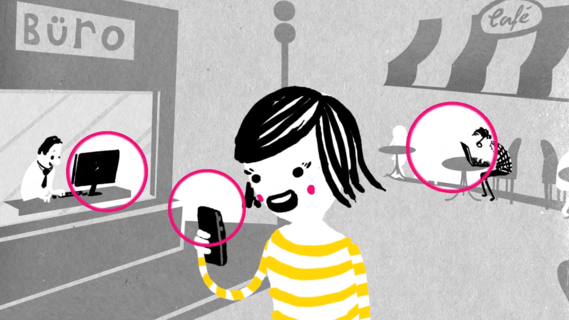
\includegraphics[width=\paperwidth]{../images/city_center}
\end{center}

\vspace{0.8cm}

\begin{Row}
    \begin{Cell}{5}
    \textbf{Werde ein Teil von Freifunk} \\
Freifunk-Netze sind Selbstmach-Netze. Auch du kannst mit einfachen Mitteln dazu
 beitragen, indem du einen Teil deiner Netzwerkressourcen anderen zur Verfügung
 stellst. Wenn viele mitmachen, entsteht ein flächendeckendes freies WLAN-Netzwerk in Darmstadt.
    \end{Cell}
    \begin{Cell}{4}
    \textbf{Wir verstehen frei als:} \vspace*{-0.18cm}
	\begin{itemize}
	   \item[\textcolor{freifunkpink}{\Large$\bullet$}] öffentlich \vspace*{-0.3cm}
	   \item[\textcolor{freifunkpink}{\Large$\bullet$}] anonym zugänglich \vspace*{-0.3cm}
	   \item[\textcolor{freifunkpink}{\Large$\bullet$}] nicht kommerziell \vspace*{-0.3cm}
	   \item[\textcolor{freifunkpink}{\Large$\bullet$}] unzensiert \vspace*{-0.3cm}
	   \item[\textcolor{freifunkpink}{\Large$\bullet$}] gemeinschaftlich betrieben\vspace*{-0.3cm}
	   \item[\textcolor{freifunkpink}{\Large$\bullet$}] und dezentral organisiert
	\end{itemize}
    \end{Cell}
\end{Row}
\newpage

\thispagestyle{empty}

\begin{Row}[cellsep=0.75cm]
    \begin{Cell}{4}
    \textbf{Was kann man damit tun?} \\
    Durch Freifunk werden z.B. lizenzfreies Community-Radio, die Übertragung lokaler Events, Telefonieren, Chatten, der Austausch öffentlicher Dateien und die gemeinsame Nutzung eines Internetanschlusses möglich.
    \end{Cell}
\begin{Cell}{5}
    \textbf{Kein rechtliches Risiko für dich} \\
Freifunk Darmstadt hilft dir dabei, ein passendes Gerät zu finden und einzurichten. Dieser sogenannte Freifunkknoten leitet den Datenverkehr über die Freifunk-Server ins Internet. Dadurch kann der Datenverkehr anderer nicht auf deine Verbindung zurückgeführt werden.
\end{Cell}
\end{Row}

\vspace{1.3cm}
\begin{Row}
    \begin{Cell}{1}
	Wenn du mit uns zusammenarbeiten möchtest, dann komm bei unseren wöchentlichen Treffen vorbei.
	\end{Cell}
\end{Row}
\vspace{0.5cm}
\begin{center}
	\large Termine und Kontakte findest du unter \\
	\url{darmstadt.freifunk.net}
\end{center}
\begin{center}
\vspace{-0.5cm}
\hspace*{-0.05 \paperwidth}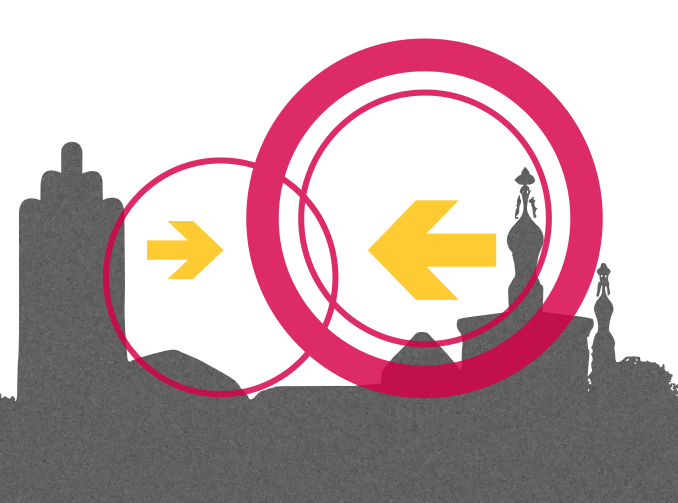
\includegraphics[width=\paperwidth]{../images/logo_skyline_large}

\vspace{-2.7cm}
\large \textcolor{lightgrey}{Twitter: \textit{@freifunkda}}
\end{center}
\end{document}
